\chapter{Noções de topologia}

A seguir introduzimos brevemente os conceitos de norma e conjunto aberto em \(\R^2\), estes generalizam as ideias de \textit{módulo} e de \textit{intervalo aberto}, isto nos dará condições de definir pontos de acumulação em \(\R^2\).

\section{O espaço vetorial \texorpdfstring{\(\R^2\)}{R2}}

Denotamos \[\R^2 = \R \times \R = \{(x,y): x,y\in\R\},\] e fixamos no plano um sistema ortogonal de coordenadas cartesianas identificando o ponto \(P = (x,y)\) ao vetor \(\overrightarrow{OP}\), com \(O = (0,0)\) sendo a origem do sistema e indicamos por \(\overrightarrow{i} = (1,0)\) e \(\overrightarrow{j} = (0,1)\). Com essa notação, \(\overrightarrow{OP} = x\overrightarrow{i} + y\overrightarrow{j}\).
        \begin{figure}[htbp]
            \centering
                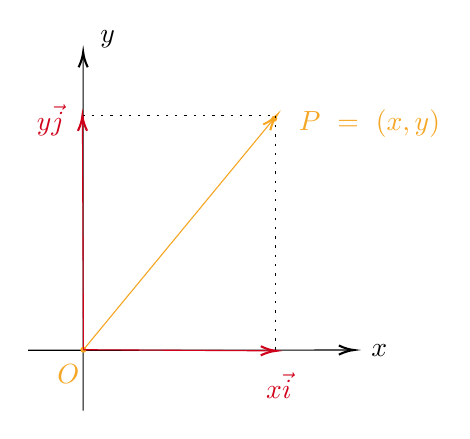
\begin{tikzpicture}[x=0.5pt,y=0.5pt,yscale=-1,xscale=1]
                    %Straight Lines [id:da4159098337804338] 
                    \draw    (104.71,287.51) -- (104.7,30.34) ;
                    \draw [shift={(104.7,28.34)}, rotate = 90] [color={rgb, 255:red, 0; green, 0; blue, 0 }  ][line width=0.75]    (10.93,-3.29) .. controls (6.95,-1.4) and (3.31,-0.3) .. (0,0) .. controls (3.31,0.3) and (6.95,1.4) .. (10.93,3.29)   ;
                    %Straight Lines [id:da3871609262592184] 
                    \draw    (64.99,243.82) -- (298.42,243.63) ;
                    \draw [shift={(300.42,243.63)}, rotate = 179.95] [color={rgb, 255:red, 0; green, 0; blue, 0 }  ][line width=0.75]    (10.93,-3.29) .. controls (6.95,-1.4) and (3.31,-0.3) .. (0,0) .. controls (3.31,0.3) and (6.95,1.4) .. (10.93,3.29)   ;
                    %Shape: Circle [id:dp11694751162050443] 
                    \draw  [draw opacity=0][fill={rgb, 255:red, 245; green, 166; blue, 35 }  ,fill opacity=1 ] (102.71,243.41) .. controls (102.71,242.21) and (103.68,241.23) .. (104.89,241.23) .. controls (106.1,241.23) and (107.07,242.21) .. (107.07,243.41) .. controls (107.07,244.62) and (106.1,245.6) .. (104.89,245.6) .. controls (103.68,245.6) and (102.71,244.62) .. (102.71,243.41) -- cycle ;
                    %Shape: Ellipse [id:dp18096494615025838] 
                    \draw  [draw opacity=0][fill={rgb, 255:red, 245; green, 166; blue, 35 }  ,fill opacity=1 ] (240.61,76.46) .. controls (240.61,75.26) and (241.59,74.28) .. (242.79,74.28) .. controls (244,74.28) and (244.98,75.26) .. (244.98,76.46) .. controls (244.98,77.67) and (244,78.64) .. (242.79,78.64) .. controls (241.59,78.64) and (240.61,77.67) .. (240.61,76.46) -- cycle ;
                    %Straight Lines [id:da627596661900103] 
                    \draw [color={rgb, 255:red, 245; green, 166; blue, 35 }  ,draw opacity=1 ]   (104.89,243.41) -- (243.07,75.82) ;
                    \draw [shift={(244.34,74.28)}, rotate = 129.51] [color={rgb, 255:red, 245; green, 166; blue, 35 }  ,draw opacity=1 ][line width=0.75]    (10.93,-3.29) .. controls (6.95,-1.4) and (3.31,-0.3) .. (0,0) .. controls (3.31,0.3) and (6.95,1.4) .. (10.93,3.29)   ;
                    %Straight Lines [id:da7299820646489661] 
                    \draw  [dash pattern={on 0.84pt off 2.51pt}]  (104.16,74.28) -- (243.97,74.28) ;
                    %Straight Lines [id:da9011614234160601] 
                    \draw  [dash pattern={on 0.84pt off 2.51pt}]  (243.97,74.28) -- (243.97,244.25) ;
                    %Straight Lines [id:da46898590550228836] 
                    \draw [color={rgb, 255:red, 208; green, 2; blue, 27 }  ,draw opacity=1 ]   (104.89,243.41) -- (241.97,244.23) ;
                    \draw [shift={(243.97,244.25)}, rotate = 180.34] [color={rgb, 255:red, 208; green, 2; blue, 27 }  ,draw opacity=1 ][line width=0.75]    (10.93,-3.29) .. controls (6.95,-1.4) and (3.31,-0.3) .. (0,0) .. controls (3.31,0.3) and (6.95,1.4) .. (10.93,3.29)   ;
                    %Straight Lines [id:da6818022320100449] 
                    \draw [color={rgb, 255:red, 208; green, 2; blue, 27 }  ,draw opacity=1 ]   (104.89,243.41) -- (104.17,76.28) ;
                    \draw [shift={(104.16,74.28)}, rotate = 89.75] [color={rgb, 255:red, 208; green, 2; blue, 27 }  ,draw opacity=1 ][line width=0.75]    (10.93,-3.29) .. controls (6.95,-1.4) and (3.31,-0.3) .. (0,0) .. controls (3.31,0.3) and (6.95,1.4) .. (10.93,3.29)   ;

                    % Text Node
                    \draw (311.05,238.14) node [anchor=north west][inner sep=0.75pt]  [font=\normalsize]  {$x$};
                    % Text Node
                    \draw (115.29,11.07) node [anchor=north west][inner sep=0.75pt]  [font=\normalsize]  {$y$};
                    % Text Node
                    \draw (84.12,252.25) node [anchor=north west][inner sep=0.75pt]    {$\textcolor[rgb]{0.96,0.65,0.14}{O}$};
                    % Text Node
                    \draw (258.68,68.07) node [anchor=north west][inner sep=0.75pt]    {$\textcolor[rgb]{0.96,0.65,0.14}{P\ =\ ( x,y)}$};
                    % Text Node
                    \draw (235.09,258.21) node [anchor=north west][inner sep=0.75pt]    {$\textcolor[rgb]{0.82,0.01,0.11}{x\vec{i}}$};
                    % Text Node
                    \draw (69.37,64.45) node [anchor=north west][inner sep=0.75pt]    {$\textcolor[rgb]{0.82,0.01,0.11}{y\vec{j}}$};
                \end{tikzpicture}
            \caption{Representação do ponto-vetor \(P = (x,y)\)}
            \label{fig:pontovetor}
        \end{figure}

A partir das operações sobre vetores, esta identificação sugere como \textit{somar} pares ordenados e como \textit{multiplicar um par ordenado por um escalar}, o que motiva a seguinte definição:
    \begin{definition}
        Sejam \((x,y)\) e \((s,t)\) dois elementos quaisquer de \(\R^2\) e \(\lambda\in\R\) qualquer.
            \begin{enumerate}
                \item A \textbf{soma} (adição) de \((x,y)\) com \((s,t)\) é dada por \[(x,y) + (s,t) = (x+s,y+t),\]\index{Adição de pares ordenados}
                \item A multiplicação por escalar é definida por \[\lambda \cdot (x,y) = (\lambda\cdot x,\lambda\cdot y),\] \index{Multiplicação de um par ordenado por um escalar}
                \item A \textbf{diferença} é \[(x,y) - (s,t) = (x,y) + (-1)(s,t),\]
                \item \[(x,y) = (s,t) \Leftrightarrow x=s \text{ e } y=t.\]
            \end{enumerate}
    \end{definition}

A partir da definição acima é possível verificar as seguintes propriedades:
\begin{proposition}\label{prop.espvetorial}
    Sejam \((x,y), (s,t)\) e \((u,v)\) em \(\R^2\) e \(\alpha\) e \(\beta\) números reais quaisquer. Então valem:
        \begin{enumerate}
            \item[(A1)] \([(x,y) + (s,t)] + (u,v) = (x,y) + [(s,t)+(u,v)]\),
            \item[(A2)] \((x,y) + (s,t) = (s,t) + (x,y)\),
            \item[(A3)] \((x,y) + (0,0) = (x,y)\) \((A4) \left( (x,y) - (x,y) = (0,0) \right)\),
            \item[(M1)] \(\alpha[\beta(x,y)] = \alpha\beta(x,y)\),
            \item[(M2)] \(\alpha[(x,y)+(s,t)] = \alpha(x,y) + \alpha(s,t)\),
            \item[(M3)] \([\alpha + \beta](x,y) = \alpha(x,y) + \beta(x,y)\),
            \item[(M4)] \(1\cdot(x,y) = (x,y)\).
        \end{enumerate}
\end{proposition}

\begin{exercise}
    Mostre que, de fato, valem as propriedades enunciadas na Proposição \ref{prop.espvetorial}.
\end{exercise}

\begin{remark}
    Um conjunto \(V\) não vazio é um \textbf{espaço vetorial} quando se define em \(V\) duas operações (soma e produto por escalar) que satisfazem as oito propriedades acima.

    Dessa forma, podemos conluir que \(\R^2\) com a soma e o produto por escalar definidos acima é um espaço vetorial, seus elementos então podem ser chamados de vetores.
\end{remark}

\section{Produto escalar e perpendicularismo}

\begin{definition}
    Definimos o \textbf{produto escalar}\index{Produto escalar} entre dois vetores \((a_1,b_1)\) e \((a_2,b_2)\) por \[(a_1,b_1) \bullet (a_2,b_2) = a_1\cdot a_2 + b_1\cdot b_2.\]
\end{definition}

\begin{proposition}\label{prop.prodescalar}
    Sejam \(\overrightarrow{u} = (a_1,b_1), \overrightarrow{v} = (a_2,b_2)\) e \(\overrightarrow{w} = (a_3,b_3)\) vetores em \(\R^2\) e \(\lambda\in\R\). Então valem as seguintes propriedades do produto escalar:
        \begin{enumerate}
            \item \(\overrightarrow{u}\bullet\overrightarrow{v} = \overrightarrow{v}\bullet\overrightarrow{u}\) (comutativa)
            \item \([\overrightarrow{u} + \overrightarrow{v}]\bullet\overrightarrow{w} = \overrightarrow{u}\bullet\overrightarrow{w} + \overrightarrow{v}\overrightarrow{w}\) (distributiva)
            \item \((\lambda\overrightarrow{u})\bullet\overrightarrow{v} = \lambda(\overrightarrow{u}\bullet\overrightarrow{v}) = \overrightarrow{u}\bullet(\lambda\overrightarrow{v})\)
            \item \(\overrightarrow{u}\bullet\overrightarrow{u} \geq 0\) e \(\overrightarrow{u}\bullet\overrightarrow{u} = 0 \Leftrightarrow \overrightarrow{u}=\overrightarrow{0} = (0,0)\)
        \end{enumerate}
\end{proposition}

\begin{exercise}
    Mostre que valem as propriedades na Proposição \ref{prop.prodescalar}.
\end{exercise}

Para definirmos \textit{perpendicularismo} ou \textit{ortogonalismo} entre vetores de \(\R^2\) notamos que, para \(\overrightarrow{u} = (a_1,b_1)\) e \(\overrightarrow{v} = (a_2,b_2)\) aplicados no ponto \(P = (x,y)\in\R^2\), ou seja,
    \begin{figure}[htbp]
            \centering
                \begin{tikzpicture}[x=0.5pt,y=0.5pt,yscale=-1,xscale=1]
                   %Straight Lines [id:da8958163654346065] 
                    \draw    (124.71,290) -- (124.7,32.83) ;
                    \draw [shift={(124.7,30.83)}, rotate = 90] [color={rgb, 255:red, 0; green, 0; blue, 0 }  ][line width=0.75]    (10.93,-3.29) .. controls (6.95,-1.4) and (3.31,-0.3) .. (0,0) .. controls (3.31,0.3) and (6.95,1.4) .. (10.93,3.29)   ;
                    %Straight Lines [id:da5677242855639231] 
                    \draw    (84.99,246.31) -- (318.42,246.12) ;
                    \draw [shift={(320.42,246.12)}, rotate = 179.95] [color={rgb, 255:red, 0; green, 0; blue, 0 }  ][line width=0.75]    (10.93,-3.29) .. controls (6.95,-1.4) and (3.31,-0.3) .. (0,0) .. controls (3.31,0.3) and (6.95,1.4) .. (10.93,3.29)   ;
                    %Shape: Circle [id:dp5943062282977485] 
                    \draw  [draw opacity=0][fill={rgb, 255:red, 245; green, 166; blue, 35 }  ,fill opacity=1 ] (122.71,245.91) .. controls (122.71,244.7) and (123.68,243.72) .. (124.89,243.72) .. controls (126.1,243.72) and (127.07,244.7) .. (127.07,245.91) .. controls (127.07,247.11) and (126.1,248.09) .. (124.89,248.09) .. controls (123.68,248.09) and (122.71,247.11) .. (122.71,245.91) -- cycle ;
                    %Shape: Ellipse [id:dp5459693683014193] 
                    \draw  [draw opacity=0][fill={rgb, 255:red, 245; green, 166; blue, 35 }  ,fill opacity=1 ] (166.61,158.95) .. controls (166.61,157.75) and (167.59,156.77) .. (168.79,156.77) .. controls (170,156.77) and (170.98,157.75) .. (170.98,158.95) .. controls (170.98,160.16) and (170,161.14) .. (168.79,161.14) .. controls (167.59,161.14) and (166.61,160.16) .. (166.61,158.95) -- cycle ;
                    %Straight Lines [id:da36306957115823135] 
                    \draw    (168.79,158.95) -- (145.93,100.18) ;
                    \draw [shift={(145.2,98.32)}, rotate = 68.74] [color={rgb, 255:red, 0; green, 0; blue, 0 }  ][line width=0.75]    (10.93,-3.29) .. controls (6.95,-1.4) and (3.31,-0.3) .. (0,0) .. controls (3.31,0.3) and (6.95,1.4) .. (10.93,3.29)   ;
                    %Straight Lines [id:da99659100893396] 
                    \draw    (168.79,158.95) -- (256.4,182.06) ;
                    \draw [shift={(258.33,182.57)}, rotate = 194.77] [color={rgb, 255:red, 0; green, 0; blue, 0 }  ][line width=0.75]    (10.93,-3.29) .. controls (6.95,-1.4) and (3.31,-0.3) .. (0,0) .. controls (3.31,0.3) and (6.95,1.4) .. (10.93,3.29)   ;
                    %Shape: Arc [id:dp7366833280490898] 
                    \draw  [draw opacity=0] (167.04,155.21) .. controls (167.17,154.68) and (167.39,154.16) .. (167.71,153.68) .. controls (169.19,151.48) and (172.17,150.9) .. (174.37,152.38) .. controls (176.57,153.86) and (177.16,156.84) .. (175.68,159.04) .. controls (175.35,159.52) and (174.96,159.92) .. (174.52,160.24) -- (171.69,156.36) -- cycle ; \draw  [color={rgb, 255:red, 208; green, 2; blue, 27 }  ,draw opacity=1 ] (167.04,155.21) .. controls (167.17,154.68) and (167.39,154.16) .. (167.71,153.68) .. controls (169.19,151.48) and (172.17,150.9) .. (174.37,152.38) .. controls (176.57,153.86) and (177.16,156.84) .. (175.68,159.04) .. controls (175.35,159.52) and (174.96,159.92) .. (174.52,160.24) ;  

                    % Text Node
                    \draw (331.05,240.63) node [anchor=north west][inner sep=0.75pt]  [font=\normalsize]  {$x$};
                    % Text Node
                    \draw (135.29,13.56) node [anchor=north west][inner sep=0.75pt]  [font=\normalsize]  {$y$};
                    % Text Node
                    \draw (104.12,254.74) node [anchor=north west][inner sep=0.75pt]    {$\textcolor[rgb]{0.96,0.65,0.14}{O}$};
                    % Text Node
                    \draw (151.62,151.74) node [anchor=north west][inner sep=0.75pt]    {$\textcolor[rgb]{0.96,0.65,0.14}{P}$};
                    % Text Node
                    \draw (176.8,145.2) node [anchor=north west][inner sep=0.75pt]  [font=\tiny,color={rgb, 255:red, 208; green, 2; blue, 27 }  ,opacity=1 ]  {$\theta $};
                    % Text Node
                    \draw (134.8,77.2) node [anchor=north west][inner sep=0.75pt]    {$\vec{u}$};
                    % Text Node
                    \draw (255.3,184.2) node [anchor=north west][inner sep=0.75pt]    {$\vec{v}$};
                \end{tikzpicture}
            \caption{\(\overrightarrow{u}\) e \(\overrightarrow{v}\) no ponto \(P\)}
            \label{fig:prodescalar}
    \end{figure}
podemos mostrar que (veja \cite{guidorizzi}[pg. 103]) \[\cos(\theta) = \frac{a_1a_2 + b_1b_2}{\sqrt{a_1^2 + b_1^2}\sqrt{a_2^2b_2^2}} = \frac{(a_1,b_1)\bullet(a_2,b_2)}{\sqrt{a_1^2 + b_1^2}\sqrt{a_2^2b_2^2}}.\] Assim, é natural a seguinte definição
\begin{definition}
    Dizemos que dois vetores \((a_1,b_1)\) e \((a_2,b_2)\) são \textbf{perpendiculares} (ou ortogonais) \index{Vetores ortogonais}
\end{definition} se \[(a_1,b_1)\bullet(a_2,b_2) = 0.\]

\section{Norma de um vetor}

\begin{definition}
    A \textbf{norma}\index{Norma de um vetor} de um vetor \((x,y)\) é definida por \[\|(x,y)\| = \sqrt{x^2 + y^2}\]
\end{definition}

\begin{remark}
    \begin{enumerate}
        \item \(\|(x,y)\| = \sqrt{(x,y)\bullet(x,y)}\).
        \item A norma de \((x,y)\) é o comprimento do vetor \(\overrightarrow{OP}\)
            \begin{figure}[htbp]
            \centering
                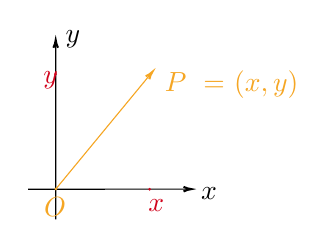
\begin{tikzpicture}[x=0.25pt,y=0.25pt,yscale=-1,xscale=1]
                   %Straight Lines [id:da8646878519160449] 
                    \draw    (124.71,290) -- (124.7,32.83) ;
                    \draw [shift={(124.7,30.83)}, rotate = 90] [color={rgb, 255:red, 0; green, 0; blue, 0 }  ][line width=0.75]    (10.93,-3.29) .. controls (6.95,-1.4) and (3.31,-0.3) .. (0,0) .. controls (3.31,0.3) and (6.95,1.4) .. (10.93,3.29)   ;
                    %Straight Lines [id:da4139533081007042] 
                    \draw    (84.99,246.31) -- (318.42,246.12) ;
                    \draw [shift={(320.42,246.12)}, rotate = 179.95] [color={rgb, 255:red, 0; green, 0; blue, 0 }  ][line width=0.75]    (10.93,-3.29) .. controls (6.95,-1.4) and (3.31,-0.3) .. (0,0) .. controls (3.31,0.3) and (6.95,1.4) .. (10.93,3.29)   ;
                    %Shape: Circle [id:dp24221391385654245] 
                    \draw  [draw opacity=0][fill={rgb, 255:red, 245; green, 166; blue, 35 }  ,fill opacity=1 ] (122.71,245.91) .. controls (122.71,244.7) and (123.68,243.72) .. (124.89,243.72) .. controls (126.1,243.72) and (127.07,244.7) .. (127.07,245.91) .. controls (127.07,247.11) and (126.1,248.09) .. (124.89,248.09) .. controls (123.68,248.09) and (122.71,247.11) .. (122.71,245.91) -- cycle ;
                    %Shape: Ellipse [id:dp7963664546761495] 
                    \draw  [draw opacity=0][fill={rgb, 255:red, 208; green, 2; blue, 27 }  ,fill opacity=1 ] (258.21,246.35) .. controls (258.21,245.15) and (259.19,244.17) .. (260.39,244.17) .. controls (261.6,244.17) and (262.58,245.15) .. (262.58,246.35) .. controls (262.58,247.56) and (261.6,248.54) .. (260.39,248.54) .. controls (259.19,248.54) and (258.21,247.56) .. (258.21,246.35) -- cycle ;
                    %Straight Lines [id:da3542526055455215] 
                    \draw [color={rgb, 255:red, 245; green, 166; blue, 35 }  ,draw opacity=1 ]   (124.89,245.91) -- (263.07,78.31) ;
                    \draw [shift={(264.34,76.77)}, rotate = 129.51] [color={rgb, 255:red, 245; green, 166; blue, 35 }  ,draw opacity=1 ][line width=0.75]    (10.93,-3.29) .. controls (6.95,-1.4) and (3.31,-0.3) .. (0,0) .. controls (3.31,0.3) and (6.95,1.4) .. (10.93,3.29)   ;
                    %Shape: Ellipse [id:dp9980659766027411] 
                    \draw  [draw opacity=0][fill={rgb, 255:red, 208; green, 2; blue, 27 }  ,fill opacity=1 ] (122.21,79.94) .. controls (122.21,78.73) and (123.19,77.75) .. (124.39,77.75) .. controls (125.6,77.75) and (126.58,78.73) .. (126.58,79.94) .. controls (126.58,81.14) and (125.6,82.12) .. (124.39,82.12) .. controls (123.19,82.12) and (122.21,81.14) .. (122.21,79.94) -- cycle ;

                    % Text Node
                    \draw (331.05,240.63) node [anchor=north west][inner sep=0.75pt]  [font=\normalsize]  {$x$};
                    % Text Node
                    \draw (135.29,13.56) node [anchor=north west][inner sep=0.75pt]  [font=\normalsize]  {$y$};
                    % Text Node
                    \draw (104.12,254.74) node [anchor=north west][inner sep=0.75pt]    {$\textcolor[rgb]{0.96,0.65,0.14}{O}$};
                    % Text Node
                    \draw (278.68,70.56) node [anchor=north west][inner sep=0.75pt]    {$\textcolor[rgb]{0.96,0.65,0.14}{P\ =\ }\textcolor[rgb]{0.96,0.65,0.14}{(}\textcolor[rgb]{0.96,0.65,0.14}{x,y}\textcolor[rgb]{0.96,0.65,0.14}{)}$};
                    % Text Node
                    \draw (254.69,257.5) node [anchor=north west][inner sep=0.75pt]    {$\textcolor[rgb]{0.82,0.01,0.11}{x}$};
                    % Text Node
                    \draw (102.97,72.94) node [anchor=north west][inner sep=0.75pt]    {$\textcolor[rgb]{0.82,0.01,0.11}{y}$};
                \end{tikzpicture}
            \caption{\(\overrightarrow{u}\) e \(\overrightarrow{v}\) no ponto \(P\)}
            \label{fig:prodescalar}
            \end{figure}
    \end{enumerate}
\end{remark}

Podemos mostra os seguintes resultados relacionados à norma de um vetor.

\begin{theorem}[Desigualdade de Schwarz]
    Dados dois vetores \(\overrightarrow{u}\) e \(\overrightarrow{v}\) de \(\R^2\) quaisquer, temos \[|\overrightarrow{u}\bullet\overrightarrow{v}| \leq \|\overrightarrow{u}\|\cdot\|\overrightarrow{v}\|.\]
\end{theorem}
(Prova: \cite{guidorizzi}[pg. 109])

\begin{theorem}
    Dados \(\overrightarrow{u}\) e \(\overrightarrow{v}\) vetores de \(\R^2\) e \(\lambda\in\R\), temos
        \begin{enumerate}
            \item \(\|\overrightarrow{u}\| \geq 0\) e \(\|\overrightarrow{u}\| = 0 \Leftrightarrow \overrightarrow{u} = (0,0)\).
            \item \(\|\lambda\overrightarrow{u}\| = |\lambda|\|\overrightarrow{u}\|.\)
            \item \(\|\overrightarrow{u}+\overrightarrow{v}\| \leq \|\overrightarrow{u}\| + \|\overrightarrow{u}\|\) (Desigualdade triangular).
        \end{enumerate}
\end{theorem}
(Prova: \cite{guidorizzi}[pg. 110])

Note que a norma \(\|\cdot\|\) em \(\R^2\) se comporta como o módulo \(|\cdot|\) em \(\R\). Em particular, é fácil ver que \(\|(x,y) - (x_0,y_0)\|\) é a \textit{distância} entre os pontos \((x,y)\) e \((x_0,y_0)\).

\section{Conjuntos abertos e pontos de acumulação}

\begin{definition}
    Sejam \((x_0,y_0)\) um ponto de \(\R^2\) e \(r>0\) um número real. Chamamos o conjunto \[B_r(x_0,y_0) = \{(x,y)\in\R^2 : \|(x,y) - (x_0,y_0)\| < r\}\] de \textbf{bola aberta}\index{Bola aberta} de centro \((x_0,y_0)\) e raio \(r\).
\end{definition}

\begin{figure}[htbp]
            \centering
                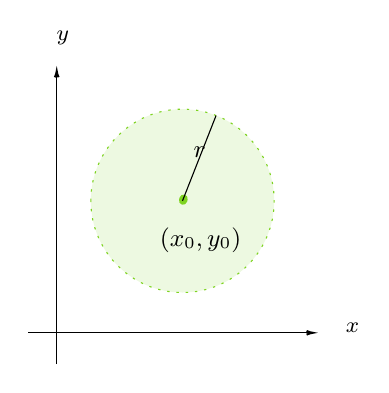
\begin{tikzpicture}[x=0.5pt,y=0.5pt,yscale=-1,xscale=1]
                    %Straight Lines [id:da8642114304094755] 
                    \draw    (246.26,267.18) -- (246.26,57.49) ;
                    \draw [shift={(246.26,55.49)}, rotate = 90] [color={rgb, 255:red, 0; green, 0; blue, 0 }  ][line width=0.75]    (4.37,-1.32) .. controls (2.78,-0.56) and (1.32,-0.12) .. (0,0) .. controls (1.32,0.12) and (2.78,0.56) .. (4.37,1.32)   ;
                    %Straight Lines [id:da3126538565319569] 
                    \draw    (225.67,244.53) -- (429.22,244.53) ;
                    \draw [shift={(431.22,244.53)}, rotate = 180] [color={rgb, 255:red, 0; green, 0; blue, 0 }  ][line width=0.75]    (4.37,-1.32) .. controls (2.78,-0.56) and (1.32,-0.12) .. (0,0) .. controls (1.32,0.12) and (2.78,0.56) .. (4.37,1.32)   ;
                    %Shape: Ellipse [id:dp40437645115208676] 
                    \draw  [color={rgb, 255:red, 126; green, 211; blue, 33 }  ,draw opacity=1 ][fill={rgb, 255:red, 184; green, 233; blue, 134 }  ,fill opacity=0.25 ][dash pattern={on 0.84pt off 2.51pt}] (270.91,149.17) .. controls (270.91,112.58) and (300.57,82.92) .. (337.16,82.92) .. controls (373.75,82.92) and (403.41,112.58) .. (403.41,149.17) .. controls (403.41,185.76) and (373.75,215.42) .. (337.16,215.42) .. controls (300.57,215.42) and (270.91,185.76) .. (270.91,149.17) -- cycle ;
                    %Shape: Free Drawing [id:dp9708220128811037] 
                    \draw  [color={rgb, 255:red, 126; green, 211; blue, 33 }  ,draw opacity=1 ][line width=3] [line join = round][line cap = round] (337.95,147.56) .. controls (337.83,148.05) and (337.7,148.54) .. (337.58,149.03) ;
                    %Straight Lines [id:da5449880117125055] 
                    \draw    (337.16,149.17) -- (361.41,87.55) ;

                    % Text Node
                    \draw (453.4,235.33) node [anchor=north west][inner sep=0.75pt]  [font=\footnotesize]  {$x$};
                    % Text Node
                    \draw (244.38,24.42) node [anchor=north west][inner sep=0.75pt]  [font=\footnotesize]  {$y$};
                    % Text Node
                    \draw (318.86,166.47) node [anchor=north west][inner sep=0.75pt]  [font=\small]  {$( x_{0} ,y_{0})$};
                    % Text Node
                    \draw (343.37,108.15) node [anchor=north west][inner sep=0.75pt]  [font=\small]  {$r$};
                \end{tikzpicture}
            \caption{Bola aberta centrada em \((x_0,y_0)\) e raio \(r\)}
            \label{fig:bolaaberta}
        \end{figure}

Note que \(B_r(x_0,y_0)\) é o conjunto de todos os pontos ``internos'' à circunferência de raio \(r\).

\begin{definition}
    Seja \(A\) um conjunto não vazio de \(R^2\). Dizemos que \((x_0,y_0)\in A\) é um \textbf{ponto interior}\index{Ponto interior} de \(A\) se \textit{existir} uma bola aberta centrada em \((x_0,y_0)\) \textit{contida} em \(A\).
\end{definition}

\begin{example}
    Seja \[A = \{(x,y)\in\R^2 : x\geq 0 \text{ e } y\geq 0\}.\]
        \begin{figure}[htbp]
            \centering
                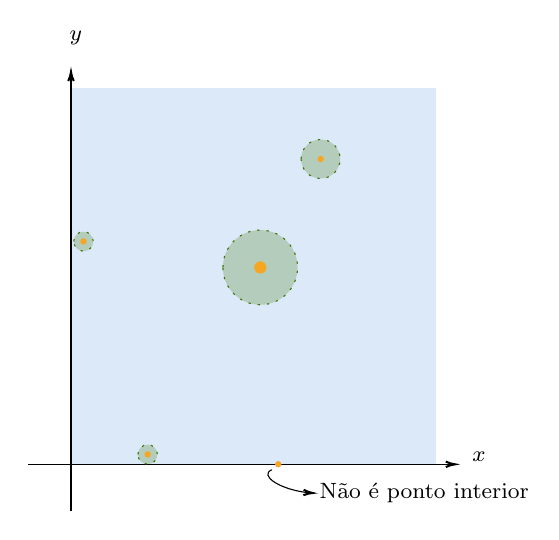
\begin{tikzpicture}[x=0.75pt,y=0.75pt,yscale=-1,xscale=1]
                    %Shape: Rectangle [id:dp8777933189090663] 
                    \draw  [draw opacity=0][fill={rgb, 255:red, 74; green, 144; blue, 226 }  ,fill opacity=0.2 ] (258.67,69.67) -- (434.87,69.67) -- (434.87,251.17) -- (258.67,251.17) -- cycle ;
                    %Shape: Circle [id:dp69142491222803] 
                    \draw  [color={rgb, 255:red, 65; green, 117; blue, 5 }  ,draw opacity=1 ][fill={rgb, 255:red, 65; green, 117; blue, 5 }  ,fill opacity=0.25 ][dash pattern={on 0.84pt off 2.51pt}] (369.8,104.07) .. controls (369.8,98.88) and (374.01,94.67) .. (379.2,94.67) .. controls (384.39,94.67) and (388.6,98.88) .. (388.6,104.07) .. controls (388.6,109.26) and (384.39,113.47) .. (379.2,113.47) .. controls (374.01,113.47) and (369.8,109.26) .. (369.8,104.07) -- cycle ;
                    %Shape: Circle [id:dp6863424862333283] 
                    \draw  [draw opacity=0][fill={rgb, 255:red, 245; green, 166; blue, 35 }  ,fill opacity=1 ] (377.67,104.07) .. controls (377.67,103.22) and (378.35,102.53) .. (379.2,102.53) .. controls (380.05,102.53) and (380.73,103.22) .. (380.73,104.07) .. controls (380.73,104.91) and (380.05,105.6) .. (379.2,105.6) .. controls (378.35,105.6) and (377.67,104.91) .. (377.67,104.07) -- cycle ;

                    %Straight Lines [id:da36860282012037626] 
                    \draw    (258.93,273.83) -- (258.93,64.13) ;
                    \draw [shift={(258.93,62.13)}, rotate = 90] [color={rgb, 255:red, 0; green, 0; blue, 0 }  ][line width=0.75]    (4.37,-1.32) .. controls (2.78,-0.56) and (1.32,-0.12) .. (0,0) .. controls (1.32,0.12) and (2.78,0.56) .. (4.37,1.32)   ;
                    %Straight Lines [id:da6280198710948994] 
                    \draw    (238.33,251.18) -- (441.89,251.18) ;
                    \draw [shift={(443.89,251.18)}, rotate = 180] [color={rgb, 255:red, 0; green, 0; blue, 0 }  ][line width=0.75]    (4.37,-1.32) .. controls (2.78,-0.56) and (1.32,-0.12) .. (0,0) .. controls (1.32,0.12) and (2.78,0.56) .. (4.37,1.32)   ;
                    %Shape: Circle [id:dp26040511917552933] 
                    \draw  [color={rgb, 255:red, 65; green, 117; blue, 5 }  ,draw opacity=1 ][fill={rgb, 255:red, 65; green, 117; blue, 5 }  ,fill opacity=0.25 ][dash pattern={on 0.84pt off 2.51pt}] (291.17,246.4) .. controls (291.17,243.8) and (293.27,241.7) .. (295.87,241.7) .. controls (298.46,241.7) and (300.57,243.8) .. (300.57,246.4) .. controls (300.57,249) and (298.46,251.1) .. (295.87,251.1) .. controls (293.27,251.1) and (291.17,249) .. (291.17,246.4) -- cycle ;
                    %Shape: Circle [id:dp12333449323387391] 
                    \draw  [draw opacity=0][fill={rgb, 255:red, 245; green, 166; blue, 35 }  ,fill opacity=1 ] (294.33,246.4) .. controls (294.33,245.55) and (295.02,244.87) .. (295.87,244.87) .. controls (296.71,244.87) and (297.4,245.55) .. (297.4,246.4) .. controls (297.4,247.25) and (296.71,247.93) .. (295.87,247.93) .. controls (295.02,247.93) and (294.33,247.25) .. (294.33,246.4) -- cycle ;
                    %Shape: Circle [id:dp19340190752565412] 
                    \draw  [draw opacity=0][fill={rgb, 255:red, 245; green, 166; blue, 35 }  ,fill opacity=1 ] (357.24,251.13) .. controls (357.24,250.28) and (357.93,249.59) .. (358.78,249.59) .. controls (359.62,249.59) and (360.31,250.28) .. (360.31,251.13) .. controls (360.31,251.97) and (359.62,252.66) .. (358.78,252.66) .. controls (357.93,252.66) and (357.24,251.97) .. (357.24,251.13) -- cycle ;
                    %Shape: Circle [id:dp9514560463314509] 
                    \draw  [color={rgb, 255:red, 65; green, 117; blue, 5 }  ,draw opacity=1 ][fill={rgb, 255:red, 65; green, 117; blue, 5 }  ,fill opacity=0.25 ][dash pattern={on 0.84pt off 2.51pt}] (260.26,143.78) .. controls (260.26,141.19) and (262.36,139.08) .. (264.96,139.08) .. controls (267.55,139.08) and (269.66,141.19) .. (269.66,143.78) .. controls (269.66,146.38) and (267.55,148.48) .. (264.96,148.48) .. controls (262.36,148.48) and (260.26,146.38) .. (260.26,143.78) -- cycle ;
                    %Shape: Circle [id:dp618587050546331] 
                    \draw  [draw opacity=0][fill={rgb, 255:red, 245; green, 166; blue, 35 }  ,fill opacity=1 ] (263.42,143.78) .. controls (263.42,142.94) and (264.11,142.25) .. (264.96,142.25) .. controls (265.8,142.25) and (266.49,142.94) .. (266.49,143.78) .. controls (266.49,144.63) and (265.8,145.32) .. (264.96,145.32) .. controls (264.11,145.32) and (263.42,144.63) .. (263.42,143.78) -- cycle ;
                    %Shape: Ellipse [id:dp7159147464909706] 
                    \draw  [color={rgb, 255:red, 65; green, 117; blue, 5 }  ,draw opacity=1 ][fill={rgb, 255:red, 65; green, 117; blue, 5 }  ,fill opacity=0.25 ][dash pattern={on 0.84pt off 2.51pt}] (332.13,156.32) .. controls (332.13,146.38) and (340.18,138.33) .. (350.12,138.33) .. controls (360.05,138.33) and (368.1,146.38) .. (368.1,156.32) .. controls (368.1,166.25) and (360.05,174.3) .. (350.12,174.3) .. controls (340.18,174.3) and (332.13,166.25) .. (332.13,156.32) -- cycle ;
                    %Shape: Ellipse [id:dp0063534561657404565] 
                    \draw  [draw opacity=0][fill={rgb, 255:red, 245; green, 166; blue, 35 }  ,fill opacity=1 ] (347.18,156.32) .. controls (347.18,154.7) and (348.5,153.38) .. (350.12,153.38) .. controls (351.74,153.38) and (353.05,154.7) .. (353.05,156.32) .. controls (353.05,157.94) and (351.74,159.25) .. (350.12,159.25) .. controls (348.5,159.25) and (347.18,157.94) .. (347.18,156.32) -- cycle ;

                    %Curve Lines [id:da9005218253794147] 
                    \draw    (355.71,253.79) .. controls (349.21,256.46) and (359.86,263.51) .. (373.38,264.84) ;
                    \draw [shift={(375.31,264.99)}, rotate = 183.18] [color={rgb, 255:red, 0; green, 0; blue, 0 }  ][line width=0.75]    (4.37,-1.32) .. controls (2.78,-0.56) and (1.32,-0.12) .. (0,0) .. controls (1.32,0.12) and (2.78,0.56) .. (4.37,1.32)   ;

                    % Text Node
                    \draw (451.07,243.98) node [anchor=north west][inner sep=0.75pt]  [font=\footnotesize]  {$x$};
                    % Text Node
                    \draw (257.05,41.07) node [anchor=north west][inner sep=0.75pt]  [font=\footnotesize]  {$y$};
                    % Text Node
                    \draw (377.47,259.07) node [anchor=north west][inner sep=0.75pt]  [font=\footnotesize] [align=left] {{Não é ponto interior}};
                \end{tikzpicture}
            \caption{\(A = \{(x,y)\in\R^2 : x\geq 0 \text{ e } y\geq 0\}.\)}
            \label{fig:retangulo}
        \end{figure}
    
        Temos:
            \begin{itemize}
                \item Todo \((x,y)\) com \(x>0\) e \(y>0\) é um ponto interior de \(A\). De fato, tome \(r = \frac{\min\{x,y\}}{2}\).
                \item Todo \((x,y)\) com \(x = 0\) ou \(y=0\) não é ponto interior de \(A\)
            \end{itemize}
\end{example}

\begin{definition}
    Seja \(A\) um subconjunto não vazio de \(\R^2\). Dizemos que \(A\) é  um \textbf{conjunto aberto}\index{Conjunto! Aberto} se todo ponto de \(A\) é interior.
\end{definition}

\begin{remark}
    Por definição \(\emptyset\) é aberto.
\end{remark}

\begin{example}
    \(A = \R^2\) é um conjunto aberto.
\end{example}

\begin{example}
    \(A = \{(x,y)\in\R^2 : x\geq 0 \text{ e } y\geq 0 \}\) não é aberto uma vez que qualquer \((x,y)\) tal que \(x=0\) ou \(y=0\) não é interior.
\end{example}

\begin{example}
    \(A = \{(x,y)\in\R^2 : x>0 \text{ e } y>0\}\) é aberto uma vez que, para qualquer \((x,y)\in A\), a bola aberta \(B_r(x,y)\subset A\) para \(r = \frac{\min\{x,y\}}{2}\).
\end{example}

\begin{example}
    Toda bola aberta é um conjunto aberto.
        
    Sejam \((x_0,y_0)\in\R^2\) e \(r>0\). Considere \(A = B_r(x_0,y_0)\) a bola aberta de centro \((x_0,y_0)\) e raio \(r\). Queremos mostrar que \(A\) é um conjunto aberto.
            \begin{figure}[htbp]
                \centering
                    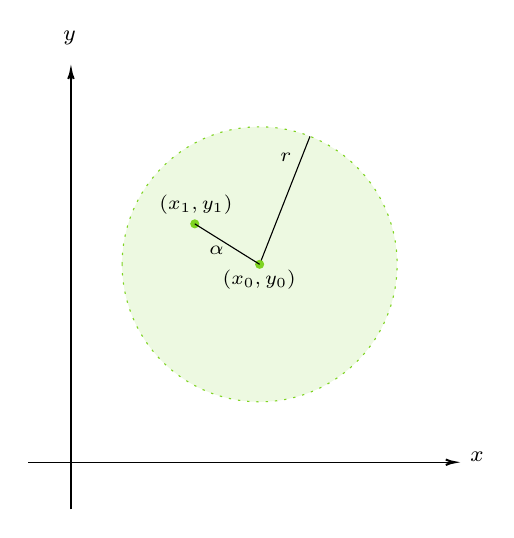
\begin{tikzpicture}[x=0.75pt,y=0.75pt,yscale=-1,xscale=1]
                        %Straight Lines [id:da28796787454131734] 
                        \draw    (62.26,279.18) -- (62.26,69.49) ;
                        \draw [shift={(62.26,67.49)}, rotate = 90] [color={rgb, 255:red, 0; green, 0; blue, 0 }  ][line width=0.75]    (4.37,-1.32) .. controls (2.78,-0.56) and (1.32,-0.12) .. (0,0) .. controls (1.32,0.12) and (2.78,0.56) .. (4.37,1.32)   ;
                        %Straight Lines [id:da4814275315650154] 
                        \draw    (41.67,256.53) -- (245.22,256.53) ;
                        \draw [shift={(247.22,256.53)}, rotate = 180] [color={rgb, 255:red, 0; green, 0; blue, 0 }  ][line width=0.75]    (4.37,-1.32) .. controls (2.78,-0.56) and (1.32,-0.12) .. (0,0) .. controls (1.32,0.12) and (2.78,0.56) .. (4.37,1.32)   ;
                        %Shape: Ellipse [id:dp6181786099110514] 
                        \draw  [color={rgb, 255:red, 126; green, 211; blue, 33 }  ,draw opacity=1 ][fill={rgb, 255:red, 184; green, 233; blue, 134 }  ,fill opacity=0.25 ][dash pattern={on 0.84pt off 2.51pt}] (86.91,161.17) .. controls (86.91,124.58) and (116.57,94.92) .. (153.16,94.92) .. controls (189.75,94.92) and (219.41,124.58) .. (219.41,161.17) .. controls (219.41,197.76) and (189.75,227.42) .. (153.16,227.42) .. controls (116.57,227.42) and (86.91,197.76) .. (86.91,161.17) -- cycle ;
                        %Straight Lines [id:da4126209940686475] 
                        \draw    (153.16,161.17) -- (177.41,99.55) ;
                        %Shape: Circle [id:dp5305891025346435] 
                        \draw  [draw opacity=0][fill={rgb, 255:red, 126; green, 211; blue, 33 }  ,fill opacity=1 ] (150.96,161.17) .. controls (150.96,159.95) and (151.94,158.97) .. (153.16,158.97) .. controls (154.37,158.97) and (155.36,159.95) .. (155.36,161.17) .. controls (155.36,162.38) and (154.37,163.37) .. (153.16,163.37) .. controls (151.94,163.37) and (150.96,162.38) .. (150.96,161.17) -- cycle ;
                        %Shape: Circle [id:dp32711059701265044] 
                        \draw  [draw opacity=0][fill={rgb, 255:red, 126; green, 211; blue, 33 }  ,fill opacity=1 ] (119.71,141.67) .. controls (119.71,140.45) and (120.69,139.47) .. (121.91,139.47) .. controls (123.12,139.47) and (124.11,140.45) .. (124.11,141.67) .. controls (124.11,142.88) and (123.12,143.87) .. (121.91,143.87) .. controls (120.69,143.87) and (119.71,142.88) .. (119.71,141.67) -- cycle ;
                        %Straight Lines [id:da8554113665932703] 
                        \draw    (121.91,141.67) -- (153.16,161.17) ;

                        % Text Node
                        \draw (253.4,250.33) node [anchor=north west][inner sep=0.75pt]  [font=\footnotesize]  {$x$};
                        % Text Node
                        \draw (57.38,47.42) node [anchor=north west][inner sep=0.75pt]  [font=\footnotesize]  {$y$};
                        % Text Node
                        \draw (134.11,162.72) node [anchor=north west][inner sep=0.75pt]  [font=\scriptsize]  {$( x_{0} ,y_{0})$};
                        % Text Node
                        \draw (161.87,106.15) node [anchor=north west][inner sep=0.75pt]  [font=\scriptsize]  {$r$};
                        % Text Node
                        \draw (103.61,126.47) node [anchor=north west][inner sep=0.75pt]  [font=\scriptsize]  {$( x_{1} ,y_{1})$};
                        % Text Node
                        \draw (127.65,150.95) node [anchor=north west][inner sep=0.75pt]  [font=\scriptsize]  {$\alpha $};
                \end{tikzpicture}
            \caption{\(A = B_r(x_0,y_0).\)}
            \label{fig:bolaaberta1}
            \end{figure}
    Seja \((x_1,y_1)\in B_r(x_0,y_0)\), vamos mostrar que \((x_1,y_1)\) é um ponto interior de \(B_r(x_0,y_0)\). Seja \(\alpha\) a distância de \((x_1,y_1)\) a \((x_0,y_0)\), ou seja \[\alpha = \|(x_1,y_1) - (x_0,y_0)\|\] e tome \(0 < r_1 < r-\alpha\). Afirmamos que \(B_{r_1}(x_1,y_1) \subset B_r(x_0,y_0)\). De fato, se \((x,y)\in B_{r_1}(x_1,y_1)\), então
            \begin{align*}
                \|(x,y) - (x_0,y_0)\|
                    & = \|(x,y) - (x_1,y_1) + (x_1,y_1) - (x_0,y_0)\| \\
                    & \leq \|(x,y) - (x_1,y_1)\| + \|(x_1,y_1) - (x_0,y_0)\| \\
                    & < r_1 + \alpha \\
                    & < (r-\alpha) + \alpha = r,
            \end{align*}
        ou seja, \(\|(x,y) - (x_0,y_0)\| < r\), portanto \(B_{r_1}(x_1,y_1) \subset B_r(x_0,y_0)\).
\end{example}

\begin{definition}
    Sejam \(A\) um subconjunto de \(\R^2\) e \((x_0,y_0)\in\R^2\). Dizemos que \((x_0,y_0)\) é um \textbf{ponto de acumulação}\index{Ponto de acumulação} de \(A\). Se \textit{toda} bola aberta de centro \((x_0,y_0)\) contiver pelo menos um ponto \((x,y)\in A\), com \((x,y)\neq(x_0,y_0)\).
\end{definition}

Em outras palavras, \((x_0,y_0)\) é um ponto de acumulação de \(A\) se existem pontos de \(A\), diferentes de \((x_0,y_0)\), tão próximos de \((x_0,y_0)\) quanto se queira. Observe que um ponto de acumulação pode ou não pertencer ao conjunto \(A\).

\begin{example}
    Seja \(A = \{(x,y)\in\R^2 : x>0 \text{ e } y>0\}\).
            \begin{figure}[htbp]
                \centering
                    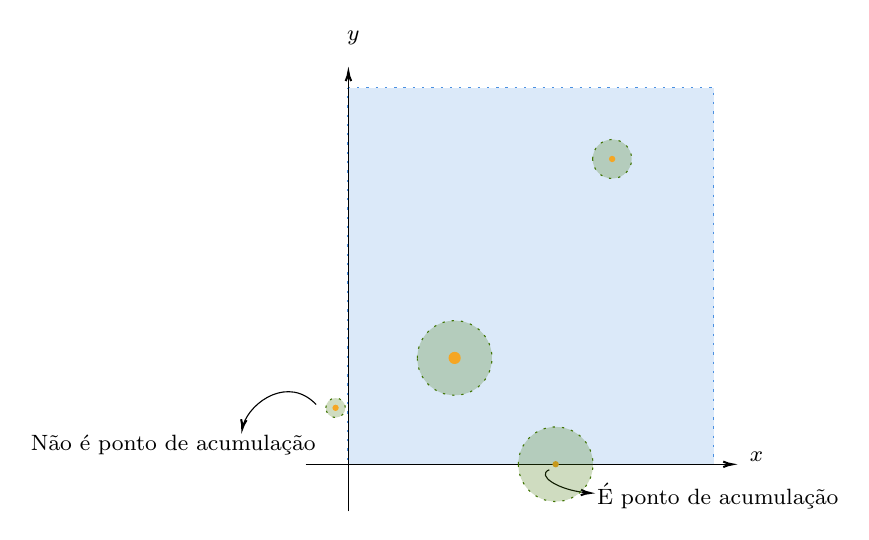
\begin{tikzpicture}[x=0.75pt,y=0.75pt,yscale=-1,xscale=1]
                        %Shape: Rectangle [id:dp26377691026360306] 
                        \draw  [color={rgb, 255:red, 74; green, 144; blue, 226 }  ,draw opacity=1 ][fill={rgb, 255:red, 74; green, 144; blue, 226 }  ,fill opacity=0.2 ][dash pattern={on 0.84pt off 2.51pt}] (217.67,73.6) -- (393.87,73.6) -- (393.87,255.1) -- (217.67,255.1) -- cycle ;
                        %Shape: Circle [id:dp010674827427814781] 
                        \draw  [color={rgb, 255:red, 65; green, 117; blue, 5 }  ,draw opacity=1 ][fill={rgb, 255:red, 65; green, 117; blue, 5 }  ,fill opacity=0.25 ][dash pattern={on 0.84pt off 2.51pt}] (335.6,108) .. controls (335.6,102.81) and (339.81,98.6) .. (345,98.6) .. controls (350.19,98.6) and (354.4,102.81) .. (354.4,108) .. controls (354.4,113.19) and (350.19,117.4) .. (345,117.4) .. controls (339.81,117.4) and (335.6,113.19) .. (335.6,108) -- cycle ;
                        %Shape: Circle [id:dp5144620491869947] 
                        \draw  [draw opacity=0][fill={rgb, 255:red, 245; green, 166; blue, 35 }  ,fill opacity=1 ] (343.47,108) .. controls (343.47,107.15) and (344.15,106.47) .. (345,106.47) .. controls (345.85,106.47) and (346.53,107.15) .. (346.53,108) .. controls (346.53,108.85) and (345.85,109.53) .. (345,109.53) .. controls (344.15,109.53) and (343.47,108.85) .. (343.47,108) -- cycle ;

                        %Straight Lines [id:da5715451905446246] 
                        \draw    (217.93,277.77) -- (217.93,68.07) ;
                        \draw [shift={(217.93,66.07)}, rotate = 90] [color={rgb, 255:red, 0; green, 0; blue, 0 }  ][line width=0.75]    (4.37,-1.32) .. controls (2.78,-0.56) and (1.32,-0.12) .. (0,0) .. controls (1.32,0.12) and (2.78,0.56) .. (4.37,1.32)   ;
                        %Straight Lines [id:da5311316382882756] 
                        \draw    (197.33,255.11) -- (400.89,255.11) ;
                        \draw [shift={(402.89,255.11)}, rotate = 180] [color={rgb, 255:red, 0; green, 0; blue, 0 }  ][line width=0.75]    (4.37,-1.32) .. controls (2.78,-0.56) and (1.32,-0.12) .. (0,0) .. controls (1.32,0.12) and (2.78,0.56) .. (4.37,1.32)   ;
                        %Shape: Circle [id:dp6421068135183269] 
                        \draw  [color={rgb, 255:red, 65; green, 117; blue, 5 }  ,draw opacity=1 ][fill={rgb, 255:red, 65; green, 117; blue, 5 }  ,fill opacity=0.25 ][dash pattern={on 0.84pt off 2.51pt}] (207.06,227.89) .. controls (207.06,225.29) and (209.16,223.19) .. (211.76,223.19) .. controls (214.35,223.19) and (216.46,225.29) .. (216.46,227.89) .. controls (216.46,230.48) and (214.35,232.59) .. (211.76,232.59) .. controls (209.16,232.59) and (207.06,230.48) .. (207.06,227.89) -- cycle ;
                        %Shape: Circle [id:dp007815117362198754] 
                        \draw  [draw opacity=0][fill={rgb, 255:red, 245; green, 166; blue, 35 }  ,fill opacity=1 ] (210.22,227.89) .. controls (210.22,227.04) and (210.91,226.36) .. (211.76,226.36) .. controls (212.6,226.36) and (213.29,227.04) .. (213.29,227.89) .. controls (213.29,228.74) and (212.6,229.42) .. (211.76,229.42) .. controls (210.91,229.42) and (210.22,228.74) .. (210.22,227.89) -- cycle ;

                        %Shape: Circle [id:dp21627777269827142] 
                        \draw  [draw opacity=0][fill={rgb, 255:red, 245; green, 166; blue, 35 }  ,fill opacity=1 ] (316.24,255.06) .. controls (316.24,254.21) and (316.93,253.53) .. (317.78,253.53) .. controls (318.62,253.53) and (319.31,254.21) .. (319.31,255.06) .. controls (319.31,255.91) and (318.62,256.59) .. (317.78,256.59) .. controls (316.93,256.59) and (316.24,255.91) .. (316.24,255.06) -- cycle ;
                        %Shape: Ellipse [id:dp7317091864212598] 
                        \draw  [color={rgb, 255:red, 65; green, 117; blue, 5 }  ,draw opacity=1 ][fill={rgb, 255:red, 65; green, 117; blue, 5 }  ,fill opacity=0.25 ][dash pattern={on 0.84pt off 2.51pt}] (251.13,203.85) .. controls (251.13,193.92) and (259.18,185.87) .. (269.12,185.87) .. controls (279.05,185.87) and (287.1,193.92) .. (287.1,203.85) .. controls (287.1,213.78) and (279.05,221.83) .. (269.12,221.83) .. controls (259.18,221.83) and (251.13,213.78) .. (251.13,203.85) -- cycle ;
                        %Shape: Ellipse [id:dp550085960004049] 
                        \draw  [draw opacity=0][fill={rgb, 255:red, 245; green, 166; blue, 35 }  ,fill opacity=1 ] (266.18,203.85) .. controls (266.18,202.23) and (267.5,200.92) .. (269.12,200.92) .. controls (270.74,200.92) and (272.05,202.23) .. (272.05,203.85) .. controls (272.05,205.47) and (270.74,206.78) .. (269.12,206.78) .. controls (267.5,206.78) and (266.18,205.47) .. (266.18,203.85) -- cycle ;
                        %Curve Lines [id:da6076630302329831] 
                        \draw    (314.71,257.72) .. controls (308.21,260.39) and (318.86,267.45) .. (332.38,268.77) ;
                        \draw [shift={(334.31,268.92)}, rotate = 183.18] [color={rgb, 255:red, 0; green, 0; blue, 0 }  ][line width=0.75]    (4.37,-1.32) .. controls (2.78,-0.56) and (1.32,-0.12) .. (0,0) .. controls (1.32,0.12) and (2.78,0.56) .. (4.37,1.32)   ;
                        %Curve Lines [id:da4254529006212977] 
                        \draw    (202.4,226.32) .. controls (189.17,212.33) and (170.94,224.78) .. (167.29,235.98) ;
                        \draw [shift={(166.8,237.92)}, rotate = 279.78] [color={rgb, 255:red, 0; green, 0; blue, 0 }  ][line width=0.75]    (4.37,-1.32) .. controls (2.78,-0.56) and (1.32,-0.12) .. (0,0) .. controls (1.32,0.12) and (2.78,0.56) .. (4.37,1.32)   ;
                        %Shape: Ellipse [id:dp08253653776412362] 
                        \draw  [color={rgb, 255:red, 65; green, 117; blue, 5 }  ,draw opacity=1 ][fill={rgb, 255:red, 65; green, 117; blue, 5 }  ,fill opacity=0.25 ][dash pattern={on 0.84pt off 2.51pt}] (299.79,255.06) .. controls (299.79,245.13) and (307.84,237.08) .. (317.78,237.08) .. controls (327.71,237.08) and (335.76,245.13) .. (335.76,255.06) .. controls (335.76,264.99) and (327.71,273.04) .. (317.78,273.04) .. controls (307.84,273.04) and (299.79,264.99) .. (299.79,255.06) -- cycle ;

                        % Text Node
                        \draw (410.07,247.91) node [anchor=north west][inner sep=0.75pt]  [font=\footnotesize]  {$x$};
                        % Text Node
                        \draw (216.05,45) node [anchor=north west][inner sep=0.75pt]  [font=\footnotesize]  {$y$};
                        % Text Node
                        \draw (336.47,263) node [anchor=north west][inner sep=0.75pt]  [font=\footnotesize] [align=left] {É ponto de acumulação};
                        % Text Node
                        \draw (63.67,239.68) node [anchor=north west][inner sep=0.75pt]  [font=\footnotesize] [align=left] {Não é ponto de acumulação};
                \end{tikzpicture}
                \caption{\(A = \{(x,y)\in\R^2 : x > 0 \text{ e } y>0\}.\)}
                \label{fig:bolaaberta2}
            \end{figure}
    
    Então, todo ponto \((x,y)\) com \(x\geq 0\) e \(y\geq 0\) é ponto de acumulação de \(A\). Em contrapartida, \(\left( -\frac{1}{2},1 \right)\) não é um ponto de acumulação (por quê?)
\end{example}

\begin{example}
    Seja \(A = \{(1,2), (-1,0), (1,3)\}\). Afirmamos que \(A\) não tem nenhum ponto de acumulação. De fato, qualquer que seja \((x_0,y_0)\in\R^2\), existe \(B_r(x_0,y_0)\) que não contém nenhum ponto de \(A\) diferente de \((x_0,y_0)\). Mais precisamente, se \((x_0,y_0)\notin A\), tome \[r < \min\{d((x_0,y_0),(1,2)), d((x_0,y_0),(-1,0)),d((x_0,y_0),(1,3))\},\] agora, se \((x_0,y_0)\in A\), basta tomar \(r = \frac{1}{2}\), por exemplo.

    \begin{remark}
        Observe que todo conjunto discreto não admite nenhum ponto de acumulação.
    \end{remark}
\end{example}

\begin{exercise}
    Qual é conjunto de todos os pontos de acumulação da bola aberta \(B_r(x_0,y_0)\)?
\end{exercise}